%%%%%%%%%%%%%%%%%%%%%%%%%%%%%%%%%%%%%%%%%%%%%%%%%%%%%%%%%%%%%%%%%%%%%%%%
\chapter{Background and Motivation}
%%%%%%%%%%%%%%%%%%%%%%%%%%%%%%%%%%%%%%%%%%%%%%%%%%%%%%%%%%%%%%%%%%%%%%%%

%%%%%%%%%%%%%%%%%%%%%%%%%%%%%%%%%%%%%%%%%%%%%%%%%%%%%%%%%%%%%%%%%%%%%%%%
\section{Graph Neural Networks}
%%%%%%%%%%%%%%%%%%%%%%%%%%%%%%%%%%%%%%%%%%%%%%%%%%%%%%%%%%%%%%%%%%%%%%%
Given a graph containing nodes, edges, and features, Graph Neural Networks (GNNs) output a per-node \textit{embedding} for each node in the graph.
An embedding is a $d$-dimensional representation of aggregated feature information from a node's neighborhood. 
Similarity in the embedding space has different meaning based on the learning task, such as similarity of node type (a node classification task) or likelihood of edge existence (a link prediction task) [todo cite]. 

In this work we will consider the case where graphs are homogeneous (one node type) and only nodes have associated features.

Borrowing notation from P3 \cite{P3_2021}, we can generally represent the embedding for a node $v$ at layer $k$ as $h_v^k$, where
\begin{align} \label{GNN Equation}
    h_v^k = \sigma \left(
         W^k \cdot 
         \mathtt{COMBINE}^{(k)} \left(
            h_v^{k-1},
            \mathtt{AGG}^{(k)} \left( 
                    \{ h_u^{k-1} \mid u \in N(v) \}
                \right) 
         \right)
     \right)
\end{align}
\begin{align*}
    \sigma &= \text{Nonlinear function} \\
    W^k &= \text{Trainable weight matrix for layer $k$} \\
    N(v) &= \text{Neighborhood of node v}
\end{align*}
$\mathtt{AGG}^{(k)}$ is a function that aggregates the previous layer embeddings of node $v$'s neighborhood. 
$\mathtt{COMBINE}^{(k)}$ is a function that combines that the result of $\mathtt{AGG}^{(k)}$ with the $v$'s own last layer embedding. 
The first layer embedding for node $v$, $h_k^0$, is just its original features.

[todo mention that this stuff is dependent on GNN architecture]

Since for each layer there is a different $W^k$, GNNs are comprised of $k$ neural networks. Furthermore, each layer requires recursive computation on a node's neighbors. Thus a \textit{$k$-hop neighborhood} must be constructed to run a $k$-layer GNN.
Generally GNNs use 1-5 layers, with 2 layers being a de facto standard \cite{Survey_First_2022}. However, some architectures can use significantly more layers, such as the current SOTA EnGCN model comprising 8 layers \cite{EnGCN_2023}.
Figure \ref{Background: GNN Execution Example} illustrates the construction of a \textit{computation graph} for a $2$-layer GNN. A computation graph describes how necessary nodes and edges participate in GNN computation.


\begin{figure}[h!]
    \begin{minipage}[c]{0.5\textwidth}
        \centering
        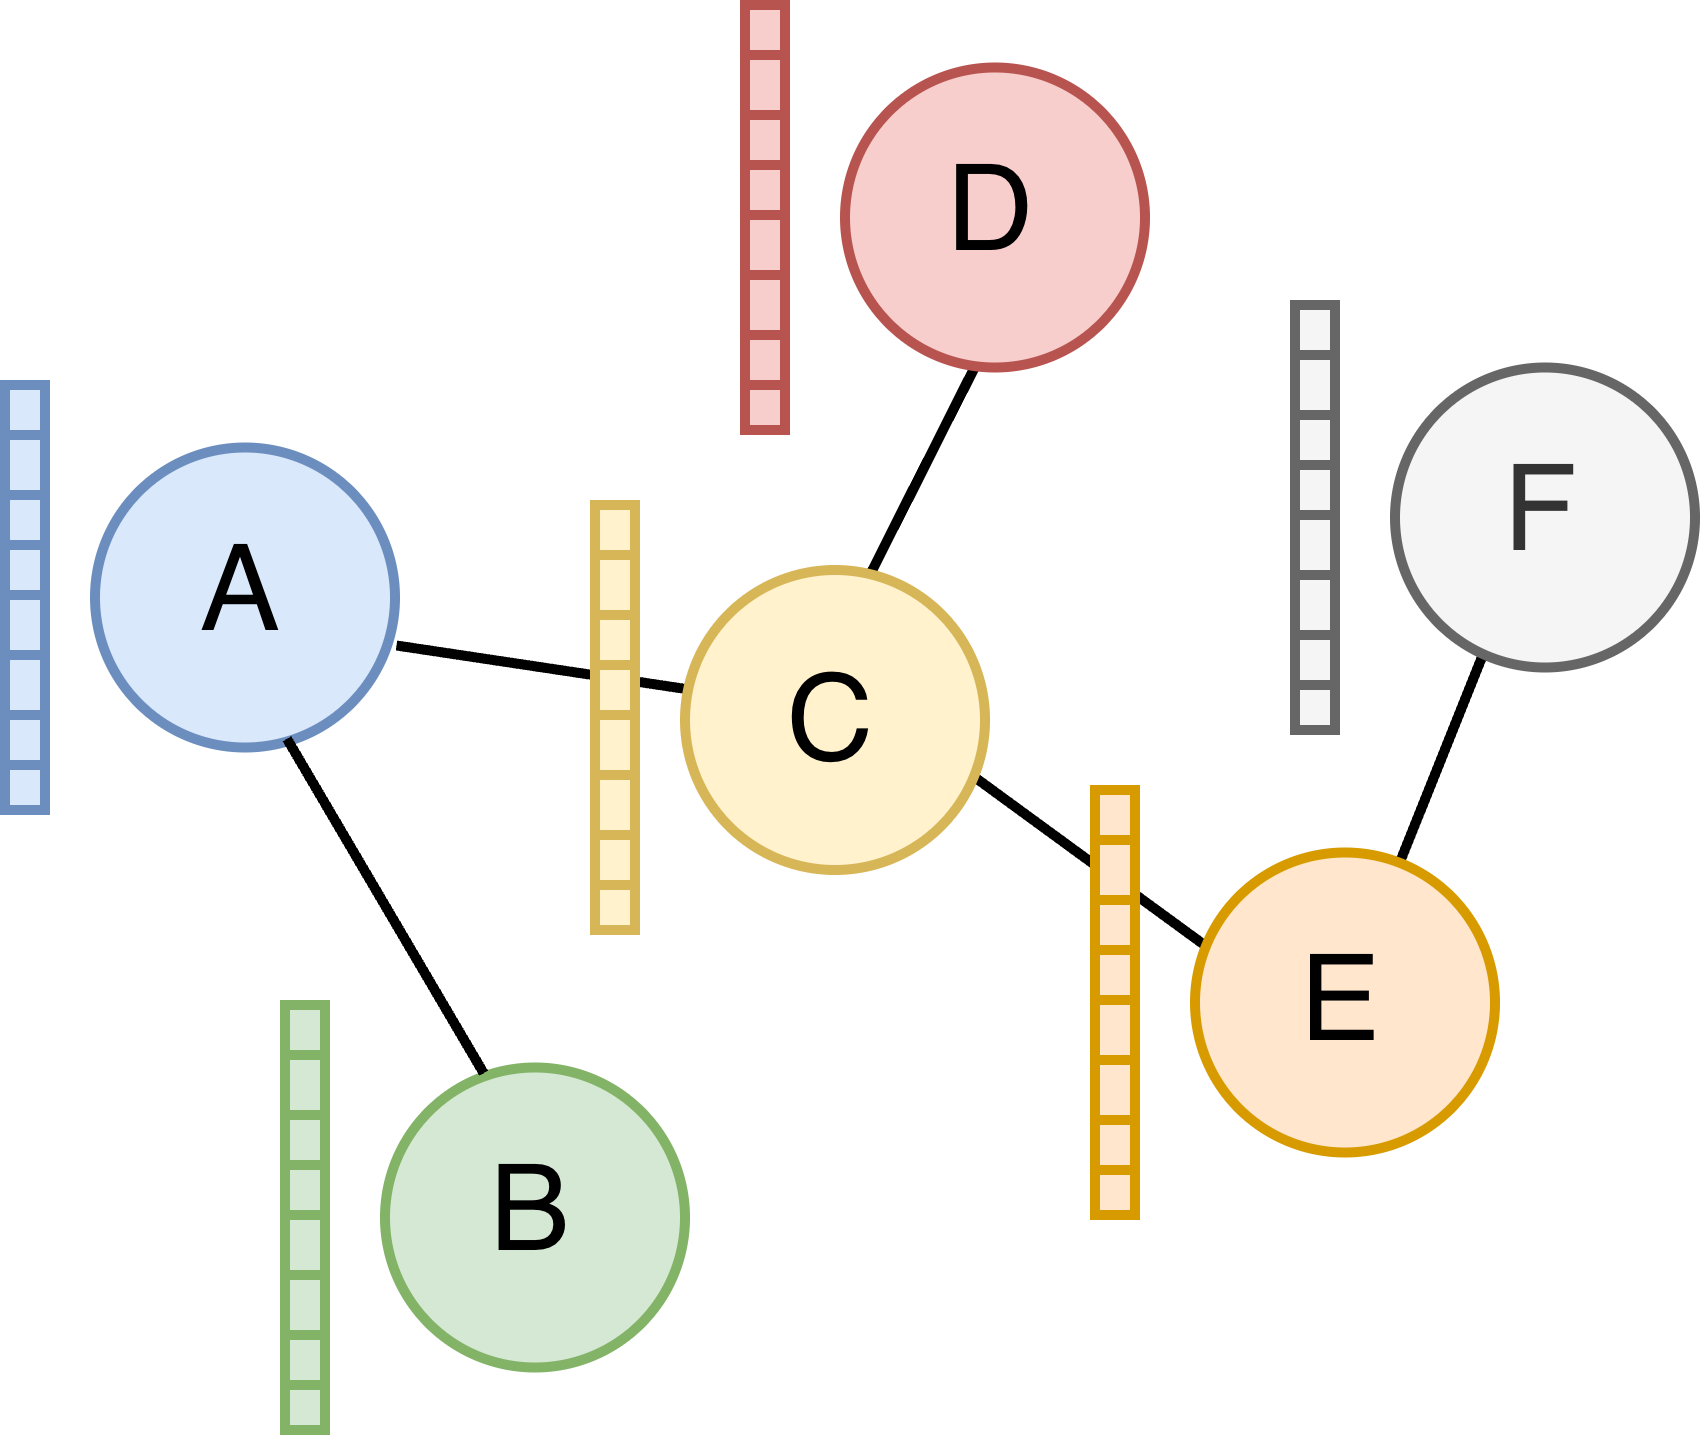
\includegraphics[width=0.85\textwidth]{diagrams/group_meeting_gnn-Graph structure.png}    
        \caption{Graph structure and associated node features (colored bars).}
    \end{minipage}
    \hfill
    \begin{minipage}[c]{0.45\textwidth}
        \centering
        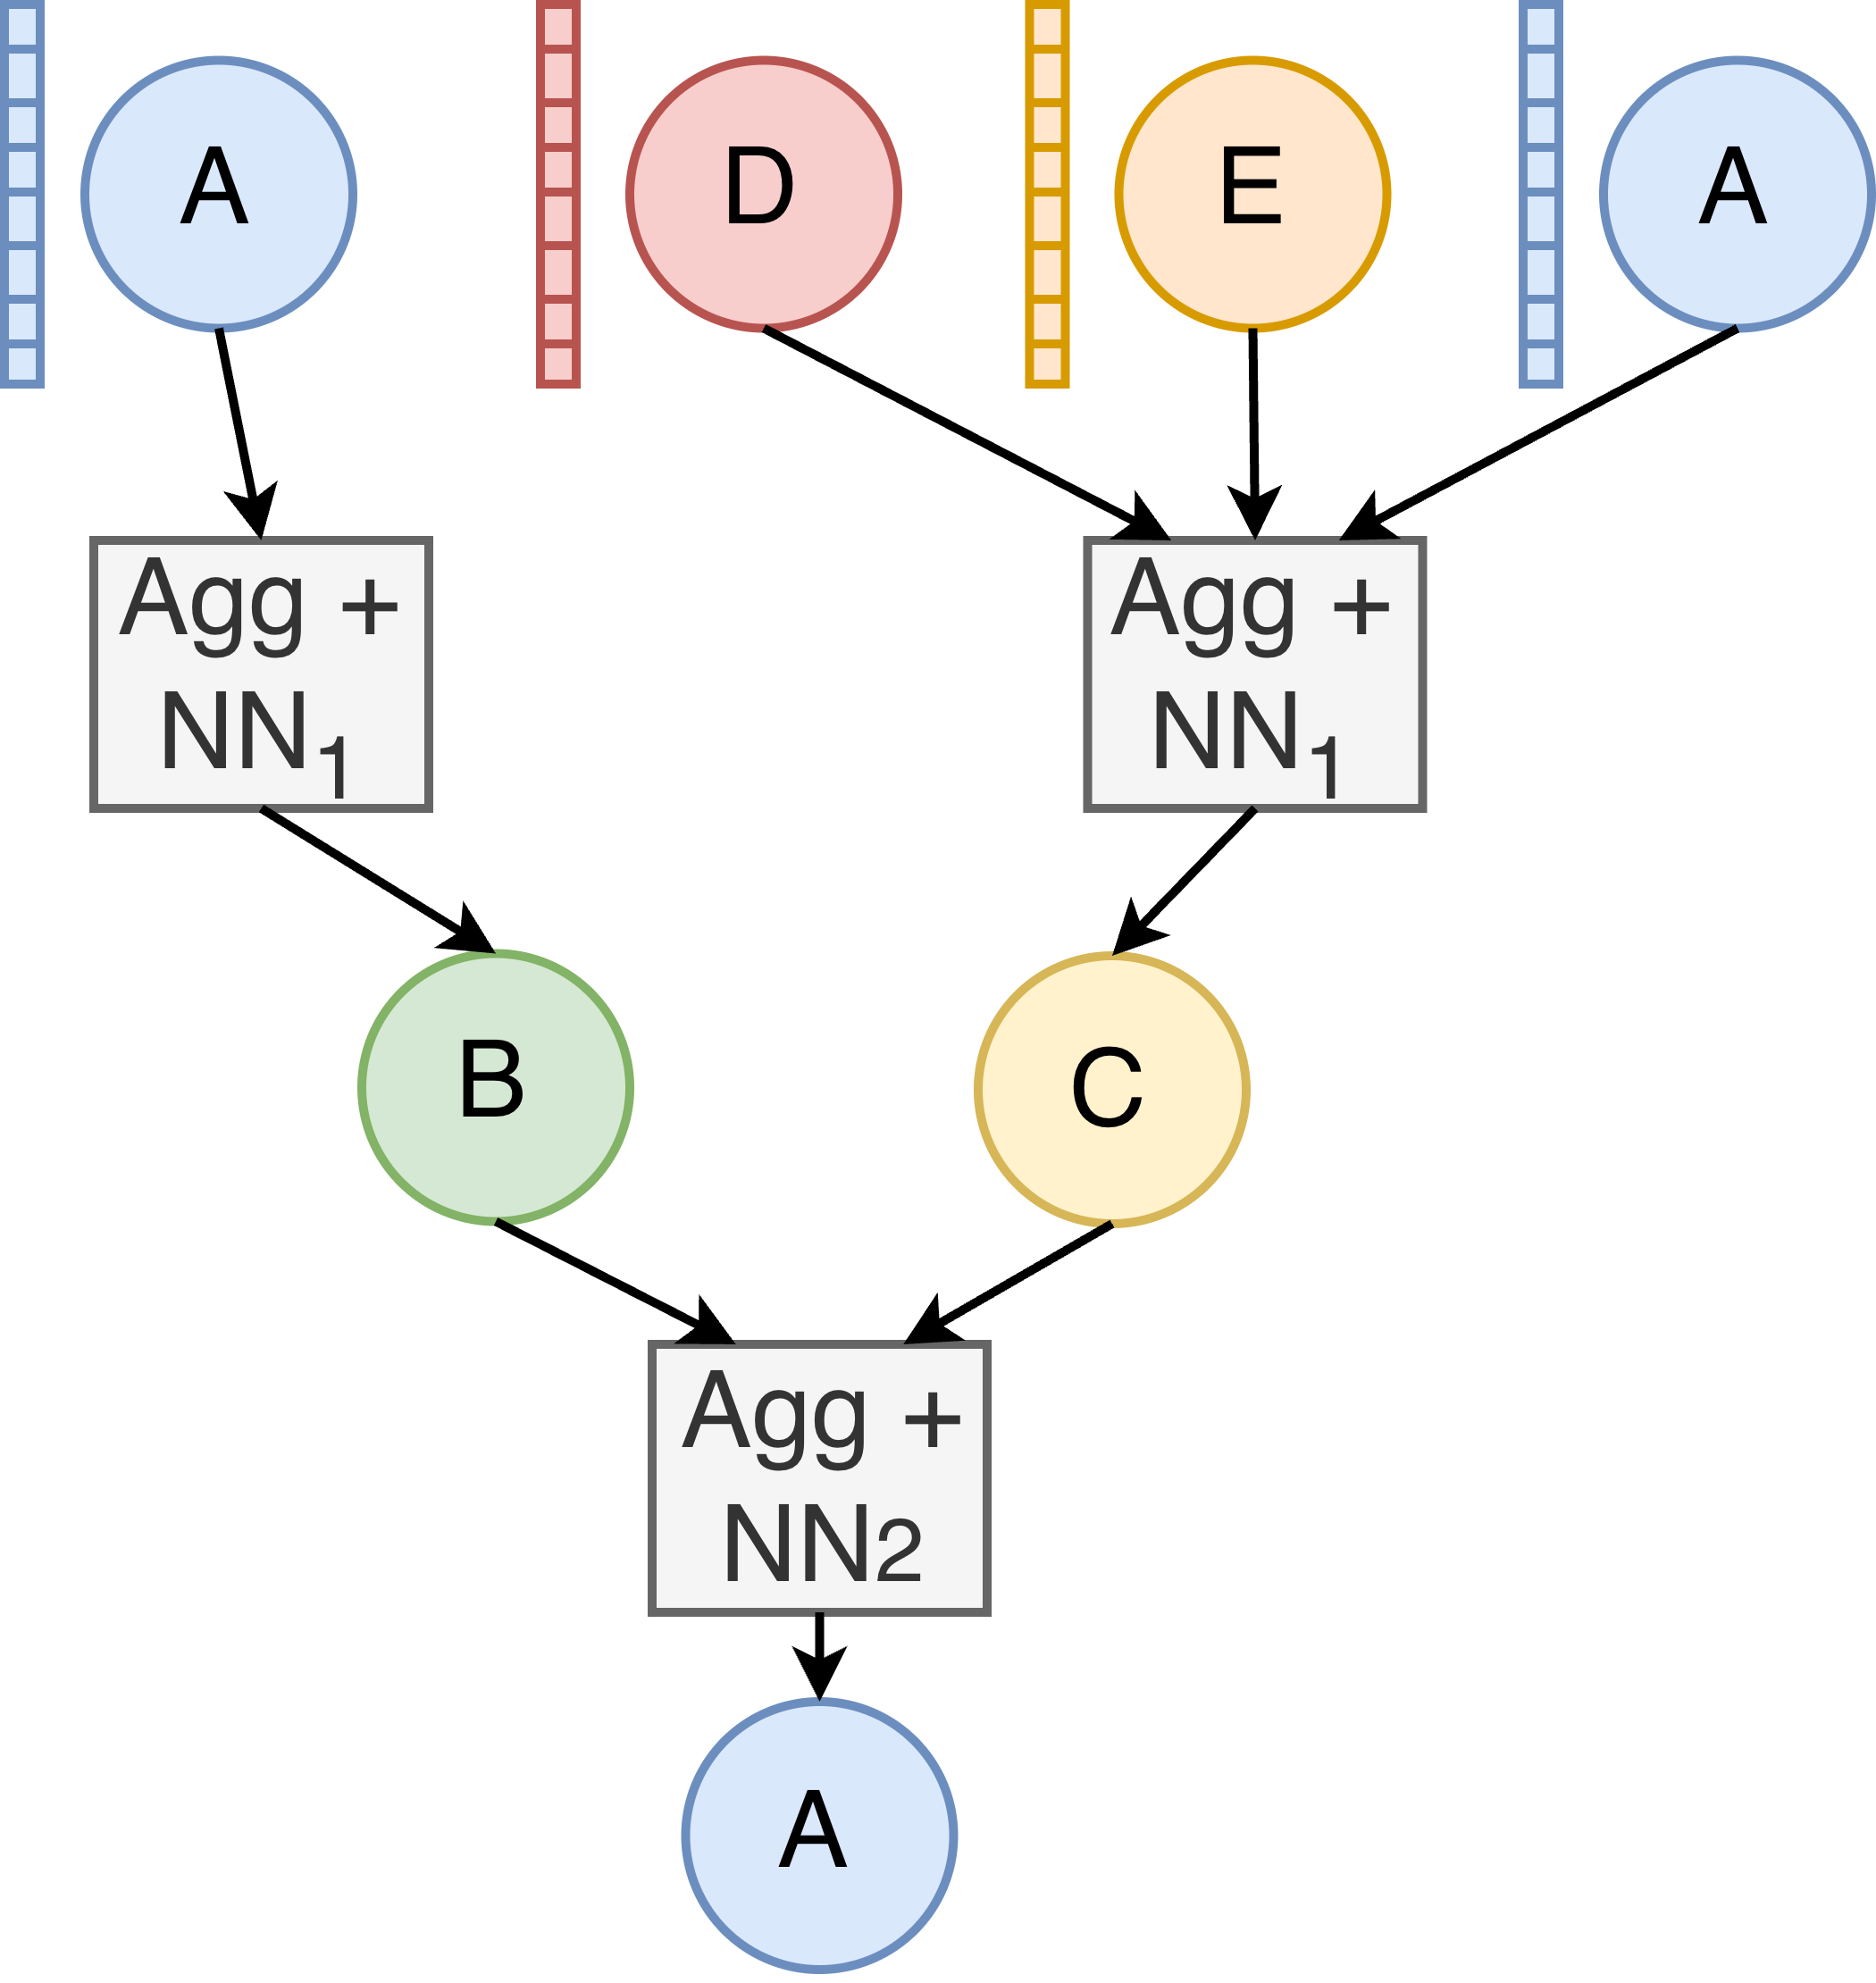
\includegraphics[width=0.95\textwidth]{diagrams/group_meeting_gnn-GNN Execution.png}
        \caption{2-hop neighborhood and computation graph for node $A$, ignoring self loops.}
    \end{minipage}
    \caption{Graph and associated computation graph for node $A$.}
    \label{Background: GNN Execution Example}
\end{figure}    

%%%%%%%%%%%%%%%%%%%%%%%%%%%%%%%%%%%%%%%%%%%%%%%%%%%%%%%%%%%%%%%%%%%%%%%%
\section{Online GNN Inference}
%%%%%%%%%%%%%%%%%%%%%%%%%%%%%%%%%%%%%%%%%%%%%%%%%%%%%%%%%%%%%%%%%%%%%%%%
Traditionally, GNN inference has been viewed as an \textit{offline} problem, where inference is performed on all nodes in the graph (full graph inference).
Full graph inference is typically used for evaluating trained models or computing node embeddings for future lookup. 
For example, PinSage \cite{Recsys_PinSAGE_2018} first uses MapReduce \cite{MapReduce_2004} to perform full graph inference before storing all node embeddings in a database.
Then, PinSage uses $K$-nearest neighbors to compute embeddings for new queries, enabling it to serve online recommendation requests.
However, this approach, along with other nearest neighbor approaches, suffers from a loss in accuracy compared to directly using a GNN to compute the new embedding.

Therefore, in this work we will view GNN inference as a \textit{online} problem, where a GNN is given a request to compute an embedding for a node or batch of nodes. In this setting, the GNN must respond to requests that consist of new nodes, their features, and edges connecting them into the existing graph.

In this section we motivate the online inference formulation and present a concrete taxonomy of the stages of GNN inference.

\subsection{Online Inference Applications}
Online inference has many applications depending on domain.
For example, in a social network graph, an inference request can correspond to computing the embedding for a new user or recomputing embeddings as a result of a new friendship. 
Furthermore, there is no strict requirement that a node is truly "new", meaning that an inference request could correspond to an update of node features.
For example, in a traffic forecasting application, an inference request can be an update of node features that represent a change in traffic conditions.

Facebook's social network graph in 2013 experienced roughly 86 thousand node or edge updates per second \cite{Graph_Survey_2020}. [todo put this in context]

\subsection{GNN Inference Stages}
While online GNN inference is generally understudied, it shares many similarities with GNN mini-batch training (discussed in Section \ref{Background: Relation to training}).

Thus when understanding the steps required to perform GNN inference, we use established taxonomy from mini-batch training work \cite{PaGraph_2020}\cite{GNNLab_2022}\cite{P3_2021}. We break down the stages of GNN inference as follows:

\begin{figure}[h!!!]
    \centering
    \begin{enumerate}
        \item \textbf{Sampling:} Construct $k$-hop neighborhood for target nodes and build logical computation graph describing GNN computation.
        \item \textbf{Data Loading:} Moving necessary data to GPU, comprising two steps.
        \begin{enumerate}
            \item \textbf{Feature gather:} Gather node features corresponding to $k$-hop neighborhood in contiguous CPU buffer.
            \item \textbf{CPU-GPU copy:} Copy buffer with node features and computation graph to GPU.
        \end{enumerate}
        \item \textbf{Model execution:} Perform GNN computation on GPU.
    \end{enumerate}
    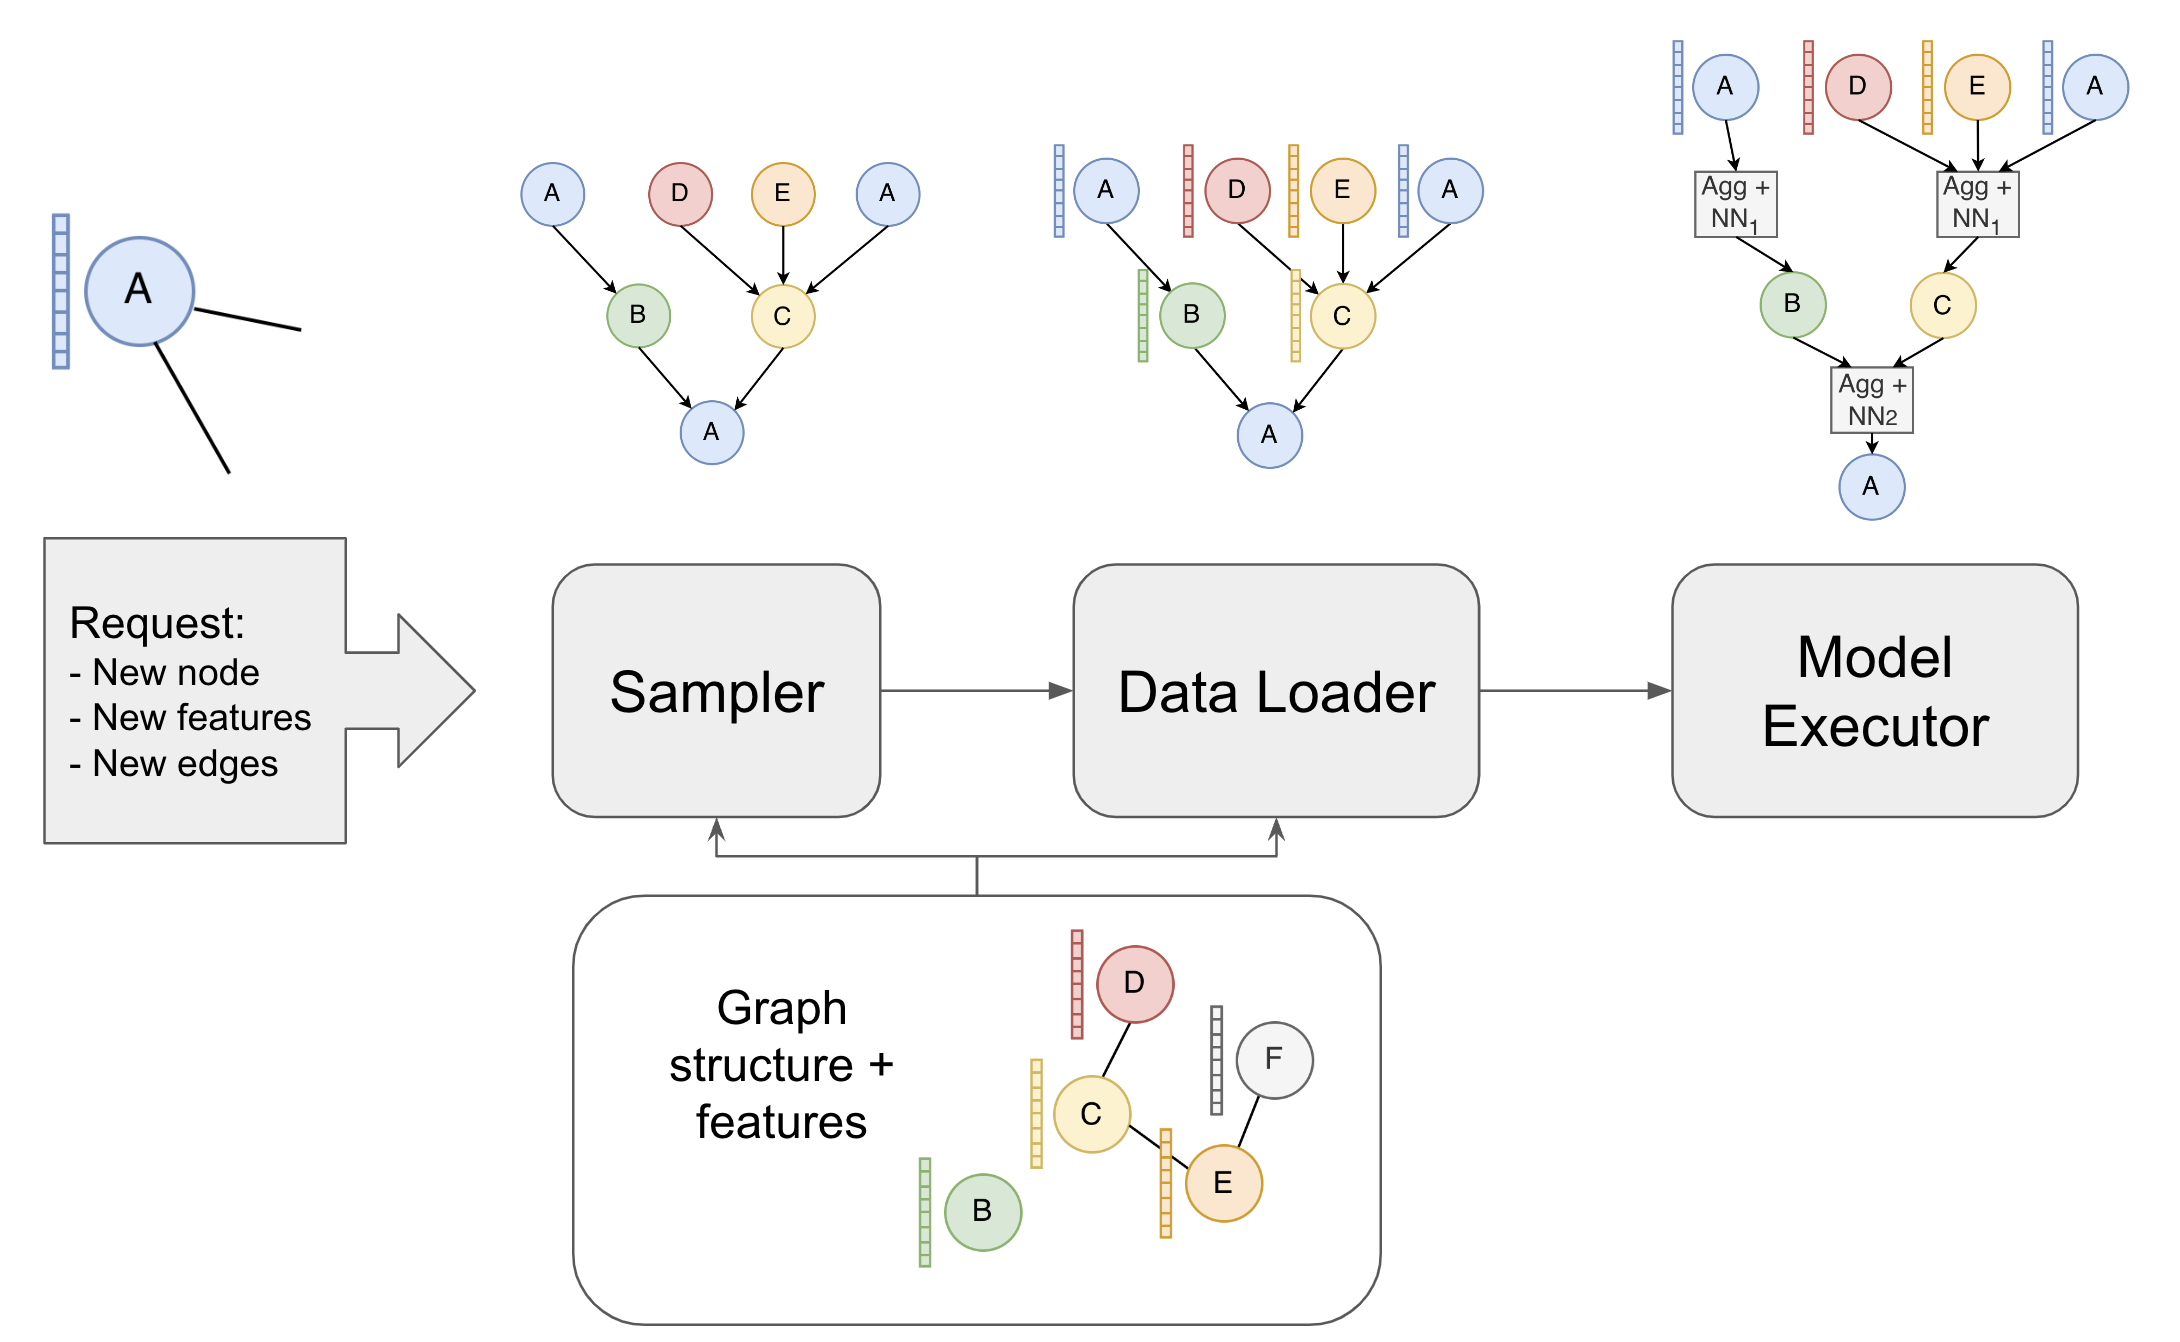
\includegraphics[width=\textwidth]{figures/Compute example.png}
    
    \caption{Online GNN Inference}
    \label{Compute Visualization}
\end{figure}    


%%%%%%%%%%%%%%%%%%%%%%%%%%%%%%%%%%%%%%%%%%%%%%%%%%%%%%%%%%%%%%%%%%%%%%%%
\section{Inference vs. Training} \label{Background: Relation to training}
%%%%%%%%%%%%%%%%%%%%%%%%%%%%%%%%%%%%%%%%%%%%%%%%%%%%%%%%%%%%%%%%%%%%%%%%
In this section we analyze similarities and differences between the inference and training tasks and examine the effectiveness of relevant GNN training optimizations at inference time.

Mini-batch training is a popular technique for GNN training on large graphs where embeddings are only computed for a random subset of the graph per epoch \cite{BGL_2023}. 
This is as opposed to full graph training, where the embeddings and gradients are computed for the entire graph at once, similar to full graph inference.
Mini-batch training is analogous to online inference, and, aside from the high-level goal, the difference is that no backpropagation is needed for inference. We briefly look at prior optimizations for the sampling and data loading stages, with particular emphasis on the latter.

\subsubsection{Sampling Optimizations}
For example, \textit{neighborhood sampling} reduces or avoids the exponential explosion in neighborhood size by randomly selecting a fixed number or percentage of node neighbors during the sampling stage \cite{GraphSAGE_2017}. 
However, since this can produce a drop in accuracy, works such as NextDoor \cite{NextDoor_2021} have proposed performing sampling on GPU rather than CPU, yielding significant speedups.
\\ \\ 
We are particularly interested in works that target the data loading stage, since movement of features from host memory to GPU memory can easily be bottlenecked by PCIe bandwidth.
A key innovation in GNN training has been caching node features in GPU memory so they no longer need to be copied over from host memory, easing data loading bottlenecks. We give a detailed treatment of three relevant works, \textbf{PaGraph}, \textbf{GNNLab}, and \textbf{BGL}.

\subsubsection{Data Loading Optimizations}

Prior GNN training works have observed that both GPU compute and memory are underutilized while training. 
\textbf{PaGraph} \cite{PaGraph_2020} used this opportunity to introduce \textit{static feature caching}, proposing a policy where the features of the highest degree nodes in the graph are stored on the GPU prior to training. 
\textbf{GNNLab} \cite{GNNLab_2022} extends static caching to include a "pre-sampling" phase, where warmup training epochs are run to determine what nodes are most often used and thus should be stored in the cache.
\textbf{BGL} \cite{BGL_2023} introduces a dynamic FIFO cache and iterates over the graph in a roughly-BFS manner to exploit the FIFO cache.
However, while these caching approaches work well for training, they are not all directly applicable to the inference case.

% However, for inference, a system can neither constrain when requests are handled nor where they reside in the graph structure. Therefore BGL's ordering based approach cannot be adapted to inference. While GNNLab's pre-sampling technique cannot be directly applied, the pre-sampling technique provides insight that a frequency based approach to identifying hot nodes is effective.

% We adapt this idea to create an online version that is suitable for inference, discussed in section [todo add a ref].

\subsection{GNN Inference Challenges}
Leveraging approaches from existing training systems present several key challenges, namely:

\begin{enumerate}
    \item \textbf{Latency is a key metric at inference time}. This is not the case during training. During training, throughput is a far more important metric than latency. For example, many training systems avoid data loading bottlenecks using pipelining. However, pipelining cannot hide latency.
    \item \textbf{Node ordering cannot be controlled}. While training systems can use 
    \item \textbf{No backpropagation leads to sampling and data loading dominating inference latency}. 
\end{enumerate}

Reasons why we optimize data lodaing stage
\begin{enumerate}
    \item \textbf{Data loading comprises 20-80\% of inference latency}
    \item \item \textbf{Data loading latency cannot be hidden with pipelining}
    \item \textbf{Data loading overhead scales with feature dimension}
\end{enumerate}


\begin{figure}[h!]
    \centering
    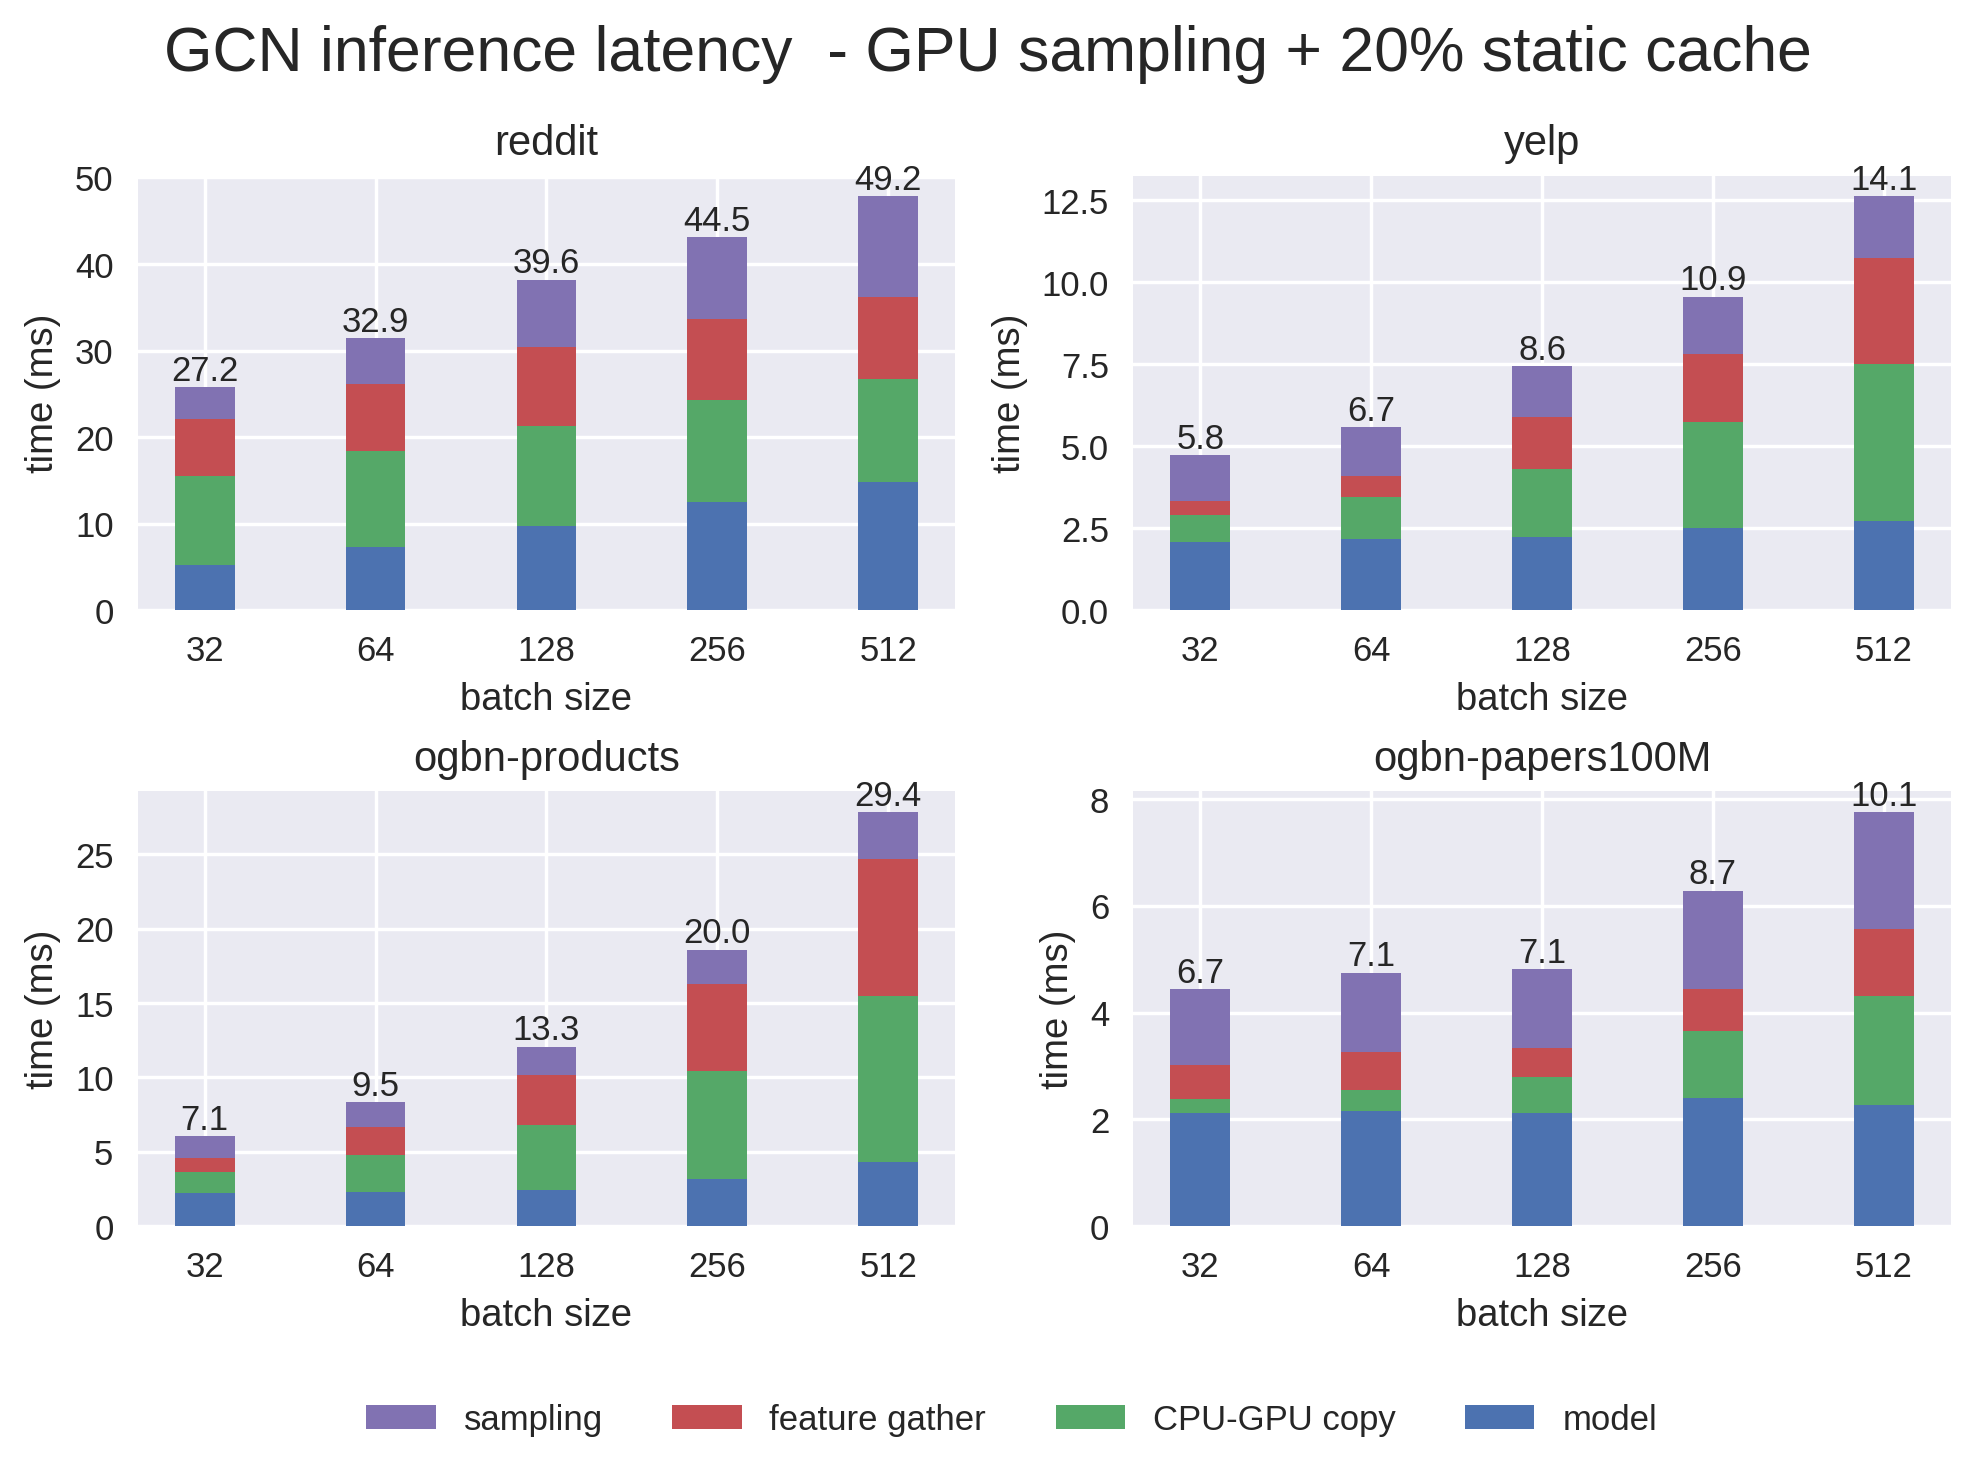
\includegraphics[width=\textwidth]{figures/GCN_latency_breakdown_gpu_sampled_with_cache.png}
    
    \caption{Inference latencies for different graph datasets and request batch sizes (number of target nodes in request). Requests are served by a system using GPU sampling and a static cache large enough to hold 20\% of the graph's node features.}
    \label{GPU Sampling Latency Breakdown}
\end{figure}    

